\chapter{INTRODUCTION}

\section{Presentation of Internship}

I conducted my internship at the Research and Data Analytics (ReDA) Lab, which is an interdisciplinary research laboratory under the Department of Applied Mathematics and Statistics at the Institute of Technology of Cambodia (ITC). This internship took place over a period of four months, from February 23rd, 2026 to June 23rd, 2026. During this time, I had the opportunity to work in a research-driven environment that focuses on Data Science, Machine Learning and Development.

ReDA Lab plays an important role as both an academic research center and an innovation hub. It brings together students, researchers, and industry partners to work on real-world problems using data-driven approaches. The lab is particularly active in developing practical solutions in areas such as analytics, AI, and applied statistics, while also encouraging student involvement in research and experimentation. Being part of this environment allowed me to not only improve my technical skills but also understand how research can be applied to real-world challenges as well.

During my internship, I worked as a Data Science Intern working on a project titled \textit{“-”} The main objective of this project was to design architectures and develop python packages that support clusterwise supervised learning and kernel-based aggregation methods. These methods are particularly useful for handling complex and heterogeneous datasets where traditional machine learning models often struggle.

Through this internship, I gained hands-on experience in both machine learning research and software development. I was involved in tasks such as studying relevant research papers on clusterwise learning and aggregation methods, designing system architecture, implementing algorithms, and evaluating models using both simulated and real-world datasets. Overall, this experience helped me bridge the gap between theoretical knowledge and practical application in the field of Data Science.

\subsection{Objective of Internship}

The main objective of this internship was to gain theoretical and practical experience in Data Science and Machine Learning by implementing and evaluating aggregation-based supervised learning methods. More specifically, the internship plays a significant role in bridging the gap between theoretical statistical learning concepts and their implementation by constructing packages for a modular machine learning library.

Particularly, the internship focuses on study, implementation, and performance assessment of several advanced ensemble and aggregation techniques, including Combine Classifier, and the KFC Procedure, followed by the redesign and modularization of these methods into a unified architecture inspired by GradientCOBRA and MixCOBRA. This restructuring aims to demonstrate that different aggregation strategies can be expressed under a common, highly extendable object oriented. Through this process, I aimed to improve my programming skills, especially in Python, as well as my ability to design clean, reusable and maintainable code at the same time.

To achieve the general objective, the internship is structured around the following specific objectives:

\begin{itemize}
    \item Studying the theoretical foundations of supervised learning, including regression and classification task and aggregation methods in improving predictive performance.
    \item Analysis of existing source code and mathematical similarities, including Combine Classifier, MixCOBRA, GradientCOBRA and KFC Procedure.
    \item Develop reusable aggregation packages under unified API interface, then empirically testing their performance.
    \item Evaluate and validate the package’s performance through extensive algorithmic experiments on both simulated and real-world datasets.
\end{itemize}


\subsection{Duration of Internship}

The internship was carried out over a period of four months, starting from February 23rd, 2026 and ending on June 23rd, 2026. During this time, I was fully engaged in research and development activities at the ReDA Lab.

This duration allowed me to progressively understand the project, starting from literature review and problem analysis, followed by implementation, testing, and evaluation of the proposed system. It also gave me enough time to gain hands-on experience and adapt to the research environment.


\section{Presentation of Organization}

\subsection{General Information of Company}

\begin{figure}[h]
    \centering
    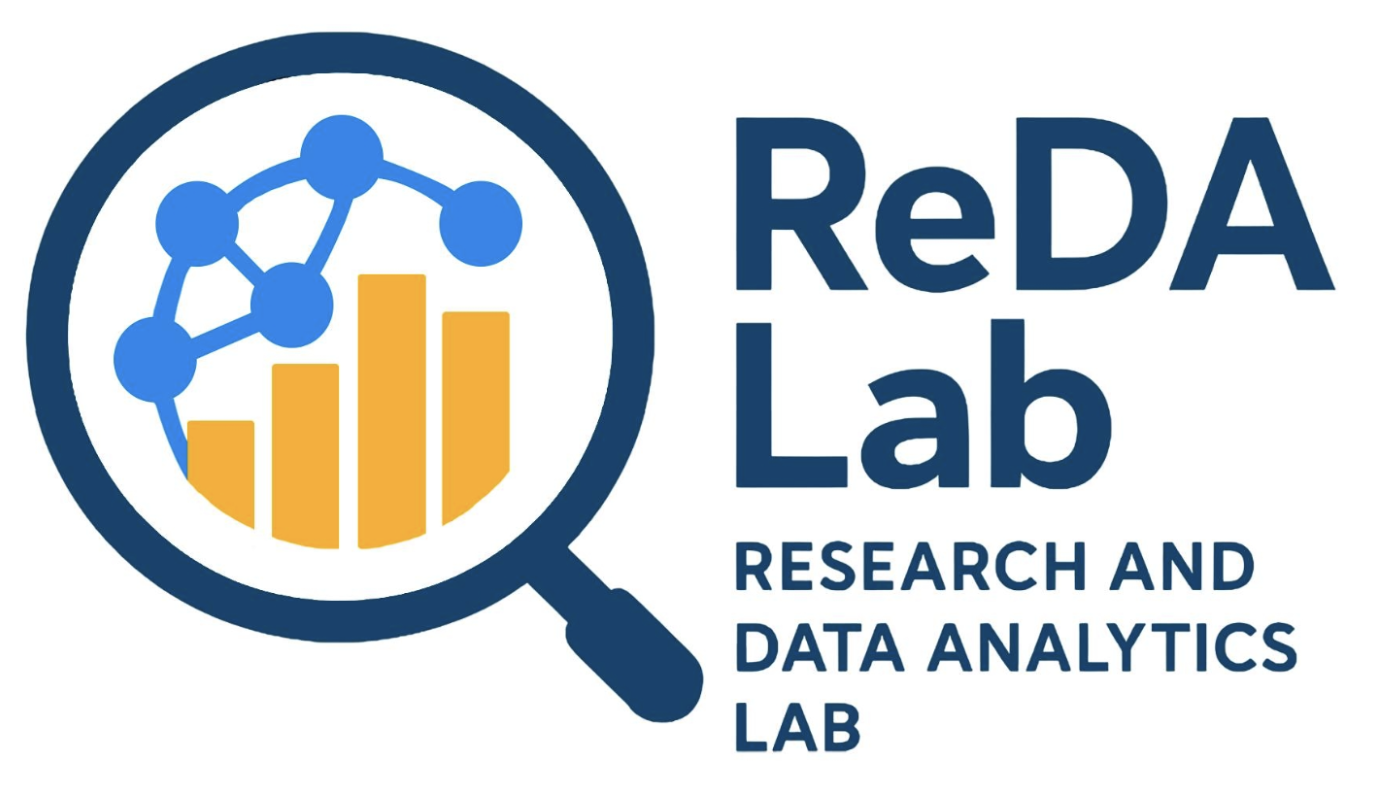
\includegraphics[width=0.6\textwidth]{figures/schools/reda-logo.png}
    \caption{ReDA Lab's Logo}
    \label{fig:reda-logo}
\end{figure}

The Research and Data Analytics (ReDA) Laboratory is the official Research and Development laboratory under the Department of Applied Mathematics and Statistics (AMS) at the Institute of Technology of Cambodia (ITC). Located at Room F201, ITC, Russian Federation Blvd (110), Phnom Penh 120404, the laboratory is dedicated to advancing research, innovation, and practical applications in Data Science, Artificial Intelligence (AI), Machine Learning, and Analytics.

ReDA Lab provides an academic and research-oriented environment where students, researchers, and faculty members collaborate on real-world projects. The laboratory supports the development of intelligent systems and data-driven solutions for education, business, industry, and public sector challenges in Cambodia. In this thesis, the research work was conducted at ReDA Lab under the supervision of the laboratory team.

\subsection{Services of Company}

ReDA Lab serves several important functions in academic research and innovation:

\begin{itemize}
    \item Academic Research Center: conducting research in Data Science, Artificial Intelligence, Computer Vision, Machine Learning, and Analytics.
    \item Research and Development Hub: developing prototypes, intelligent systems, and practical AI solutions for real-world applications.
    \item Student Innovation Platform: providing opportunities for students to participate in research projects, develop technical skills, and apply theoretical knowledge in practice.
    \item Collaboration and Knowledge Sharing Center: encouraging cooperation among students, faculty members, and external partners through structured research activities and laboratory projects.
\end{itemize}

\subsection{Vision \& Mission}

\textbf{Vision}: To become a leading research laboratory in Cambodia in the fields of Data Science, Artificial Intelligence, and Analytics, contributing to innovation, education, and sustainable national development.

\textbf{Mission}:
\begin{itemize}
    \item To conduct research and development in Artificial Intelligence, Data Science, and related fields.
    \item To promote innovation through practical and applied research projects.
    \item To provide students with opportunities to develop technical, analytical, and research skills.
    \item To collaborate with academic, industrial, and public institutions in solving real-world problems using data-driven approaches.
    \item To support the responsible and effective use of AI technologies in Cambodia.
\end{itemize}


\subsection{Organization Chart}

ReDA Lab operates under the Department of Applied Mathematics and Statistics (AMS) at the Institute of Technology of Cambodia. The laboratory is organized through a board and research-unit structure to support academic research, student innovation, and interdisciplinary collaboration. The organizational structure includes leadership roles and specialized research units such as LLM Application and Research, Computer Vision and AI, Data Science and Machine Learning, Data and Business Analytics, and Big Data and Data Engineering. This structure enables the laboratory to coordinate research activities effectively and support students in different areas of specialization.

\begin{figure}[H]
    \centering
    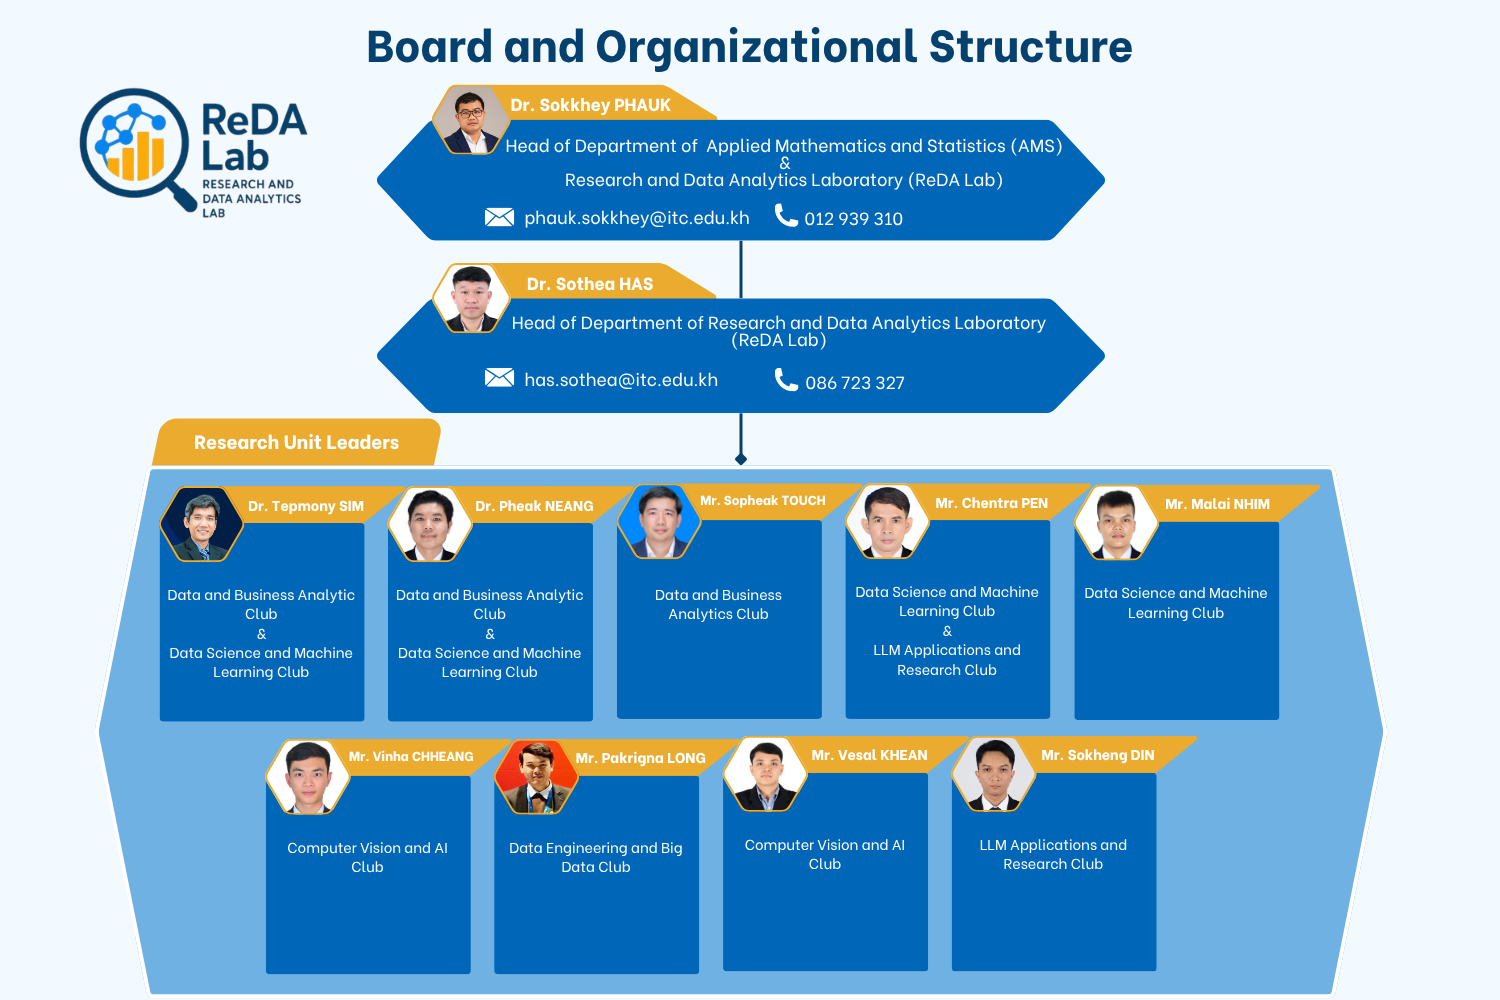
\includegraphics[width=0.6\textwidth]{figures/schools/reda-organization.png}
    \caption{ReDA Lab Board and Organizational Structure}
    \label{fig:reda-organization}
\end{figure}


\subsection{Address \& Contact}

\begin{itemize}
    \item \textbf{Organization Name:} Research and Data Analytics (ReDA) Laboratory
    \item \textbf{Institution:} Institute of Technology of Cambodia (ITC)
    \item \textbf{Department:} Department of Applied Mathematics and Statistics (AMS)
    \item \textbf{Office Location:} Room F201
    \item \textbf{Address:} Russian Federation Boulevard (110), Phnom Penh 120404, Cambodia
    \item \textbf{Contact Person:} Dr. HAS Sothea
    \item \textbf{Position:} Head of Research and Data Analytics Laboratory
    \item \textbf{Facebook:} \href{https://m.facebook.com/people/Research-and-Data-Analytics-Lab/61577145037198/}{Research and Data Analytics Lab}
\end{itemize}

\subsection{Internship Working Schedule}

During the internship, a weekly room schedule was provided by the ReDA Lab to organize workspace allocation for interns. This schedule specifies the rooms assigned for morning and afternoon sessions throughout the week, allowing efficient use of laboratory resources.

In addition to the room allocation, interns were expected to follow a fixed working schedule. For those conducting their internship exclusively at ReDA Lab, the expected presence at the laboratory was from \textbf{8:00 AM to 11:00 AM and from 1:00 PM to 4:00 PM}.

As shown in Figure ~\ref{fig:schedule}, the working rooms vary depending on the day. Most activities were conducted in rooms F309 and F201.

In addition to the regular working schedule, a weekly seminar was held every Thursday from 5:00 PM to 6:00 PM to report progress to my advisor. These sessions provided an opportunity to present ongoing work, discuss challenges, receive guidance, and review the next steps of the project.

\begin{figure}[H]
    \centering
    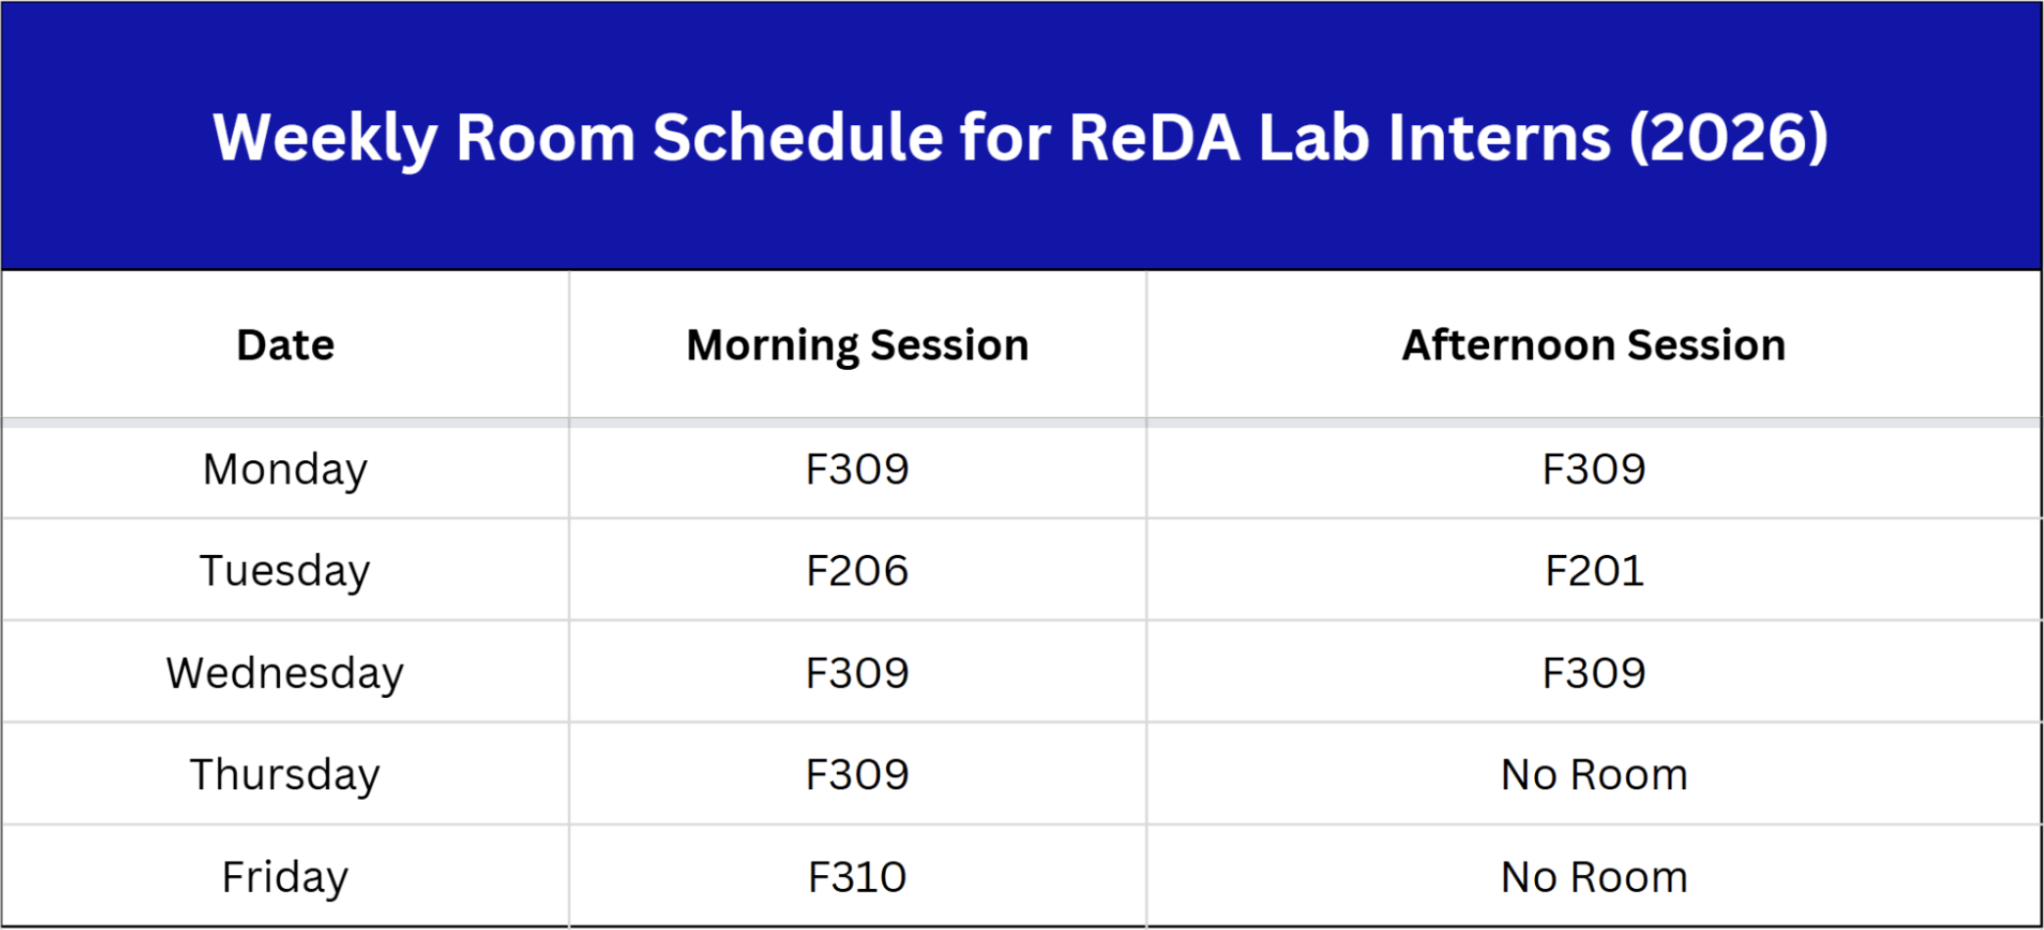
\includegraphics[width=0.6\textwidth]{figures/schools/schedule.png}
    \caption{Illustrates the weekly room schedule for ReDA Lab interns.}
    \label{fig:schedule}
\end{figure}



